Il periodo di Progettazione di dettaglio e codifica inizia con la consegna della \RP{} (2019-04-08) e termina con la consegna della \RQ{} (2019-04-19).\newline
Durante questo periodo, vengono svolte le seguenti attività:
\begin{itemize}
	\item \textbf{Modifica}: modifiche ai seguenti documenti, ove necessario:
	\begin{itemize}
		\item Piano di progetto;
		\item Piano di qualifica;
		\item Norme di progetto.
	\end{itemize}
	\item \textbf{Product Baseline}: sulla base Technology Baseline viene redatto il documento di definizione di prodotto, nella quale sono contenute le scelte progettuali di dettaglio. In particolare esso contiene:
	\begin{itemize}
		\item {\textbf{Design Pattern}}\ped{G}: tutti i design pattern impiegati all'interno del progetto;
		\item \textbf{Diagrammi di attività}: per la modellazione di un processo e l'organizzazione di più entità in un insieme di azioni secondo un determinato flusso. Adatti soprattutto all'uso con {React}\ped{G}.
		\item  \textbf{Diagrammi di classe}: diagrammi in standard UML 2.0 utilizzati per rappresentare le classi realizzate per il progetto.
	\end{itemize}
	\item \textbf{Codifica}: basandosi sulla definizione di prodotto, viene scritto il codice sorgente;
	\item \textbf{Manuale Utente}: redazione del manuale utente che definisce le modalità di utilizzo dell'applicativo, che verrà realizzato contemporaneamente allo sviluppo del codice sorgente. 
\end{itemize}
Il numero di incrementi per realizzare tali attività ha un valore fissato a 8.
\begin{figure}[H]
	\centering
	\hspace*{-1.5cm}
	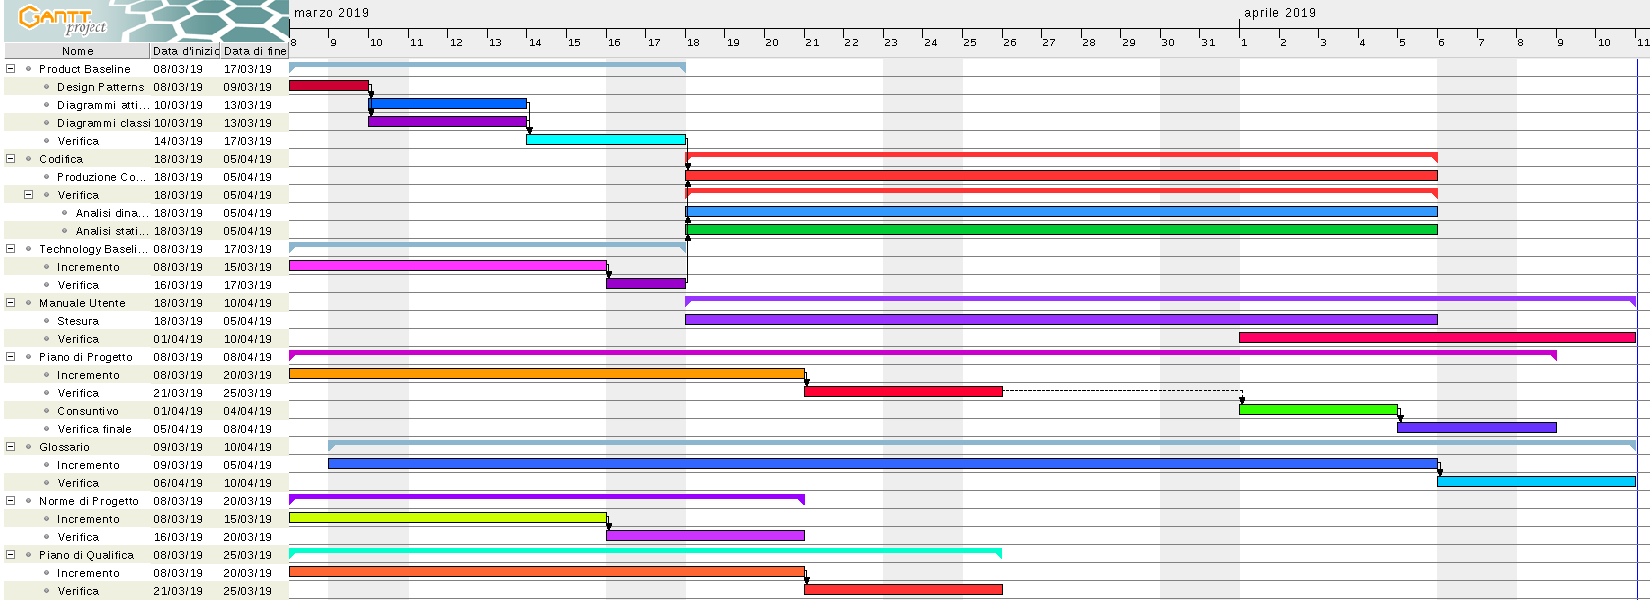
\includegraphics[width=19.4cm, height=9cm]{Pianificazione/progettazioneDettaglioCodifica.pdf}
	\caption{Diagramma di Gantt del periodo di Progettazione di dettaglio e codifica}
\end{figure}